\label{ch:enviornment}
\thcomment{I have made some major changes here. I have not removed any parts but I have removed all of the implementation details. However, I have kept some of the mathematics governing the calculation of the speed and orientation. }
\\
This chapter presents a detailed description of the environment used for \edited{conducting} the experiments. The environment, implemented using Pygame \cite{pygame}, portrays the world as a rectangular area viewed from a top-down perspective (bird's eye view). 
The size of the world can be set by altering the rows and columns during initialization. These values denote the size of the world in pixels.

The environment follows the image coordinate system: with the center at the top left corner and each position on the map is indicated by a 2-dimensional vector containing the row and column value respectively.\\
\section{Components (Re-edited entirely)}
3 key components populate the environment: 
\begin{itemize}
    \item The agent.
    \item The goal.
    \item The obstacles.
\end{itemize}
\subsection{The agent}
The agent represents the entity being controlled by an external controller. At any given moment, the state of the agent has three properties: position, speed, and orientation.
\begin{enumerate}
    \item Position: The current coordinates of the agent (in pixel coordinates) on the map.
    \item Speed: The current speed of the agent.
    \item Orientation: A unit vector along the velocity vector of the agent.
\end{enumerate}
To navigate the environment the agent can control two aspects of its motion: its speed and its orientation.
Unlike most stock environments, this supports both continuous and discrete action space. These are elaborated in \autoref{subsec:action-space}.
\subsection{The goal}
The goal is a pre-designated area of the map where on arrival marks the end of an episode with a success. It is represented by a green rectangle. Like the agent, the size of the goal area can be customized as per the requirement of the experiment. For now, the environment just has provision for static goals. That being said, the environment does come with the provision to randomly alter the position of the goal at the end of each episode.


\subsection{The obstacles}
There are 3 ways of putting obstacles in the map each of them serving a different purpose.
\begin{enumerate}
\item \textbf{Individual specification}: This is aimed at quick deployment of  a small number of static obstacles in different locations of the map and is best suited for use in the sanity check of a controller.
\item \textbf{Obstacle map}: It is the primary method of initializing static obstacles on the environment. The dimensions of the image dictate the size of the environment. The resolution of the obstacle map recreated in the environment can be adjusted as per requirement. A higher resolution portrays a obstacle map faithful to the original image, retaining finer details. The trade off to this is the large number of obstacles used to create the obstacle map which increases exponentially with the increase in resolution.
%\item \textbf{Using a list:}
%The information for the placement of the obstacles can be passed in the form of a list, where each element in the list is a Numpy array containing the pixel coordinate ([row, col]) of the obstacle. This is primarily useful when the number of obstacles to be deployed is small. Although it severely limits the number and the configuration of the obstacles that can be placed in the map, it is ideal for performing a quick initialization or a brief sanity test of a controller in a short time without investing in creating an obstacle map or an annotation file.
%\item \textbf{Using an obstacle map:}
%This is the primary way of initializing the environment with static obstacles. In this case, the path to an image file is provided during initialization. This image is then read by the environment to obtain the size of the map and the obstacle configuration. 
%The dimensions of the image determine the size of the map. Comprehending the obstacle configuration is also straight forward. Any red pixel, pixel falling in the color range of ($150$, $0$, $0$) to ($255$, $0$, $0$) is categorized as an obstacle. While defining each pixel as an individual obstacle renders the most accurate recreation of the obstacle configuration from a given image, it is inefficient as it generates an unnecessarily large number of obstacles on the map.
%This is redundant as for most of the cases, instead of having pixel-sized obstacles,  these obstacles can be grouped into bigger cells often without loosing too much information or diverging too much from the original configuration. The grouping can be adjusted by tuning the obstacle-width parameter in the environment.  Setting the width to one sets the size of an individual obstacle to $1$. This retains the highest amount of information (basically pixel-by-pixel information) from the obstacle map. Increasing the width groups pixels in the image to form obstacles of the given width, which drastically reduces the number of obstacles at the cost of introducing a pixelation effect in the final obstacle map.
%\textbf{A set of 3 images: obstacle image, and its comparison with changing obstacle size}

\begin{figure}[!h]
	\begin{subfigure}[t]{.5\textwidth}
		\centering
		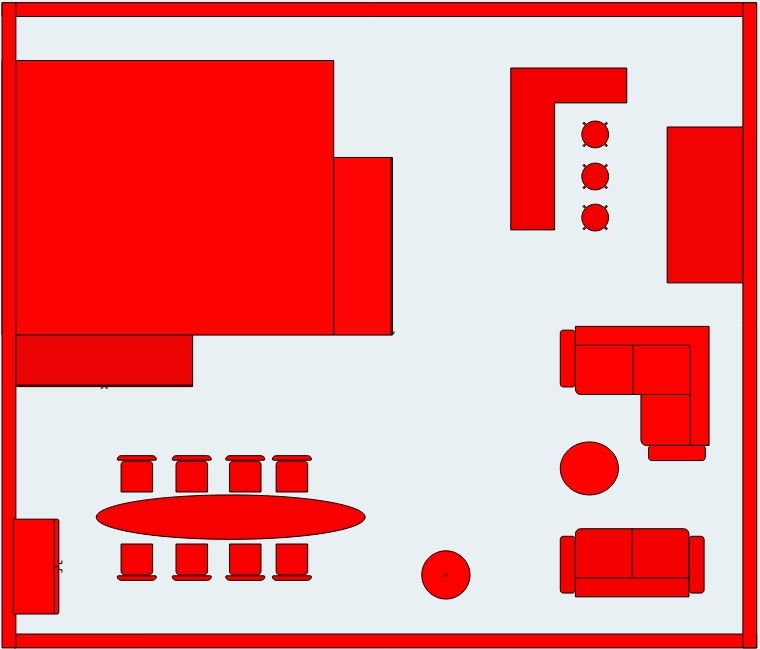
\includegraphics[width=.95\linewidth]{figures/real_map.jpg}
		\caption{The original obstacle map}
		\label{fig:obsmap_sfig1}
	\end{subfigure}%
	\begin{subfigure}[t]{.5\textwidth}
		\centering
		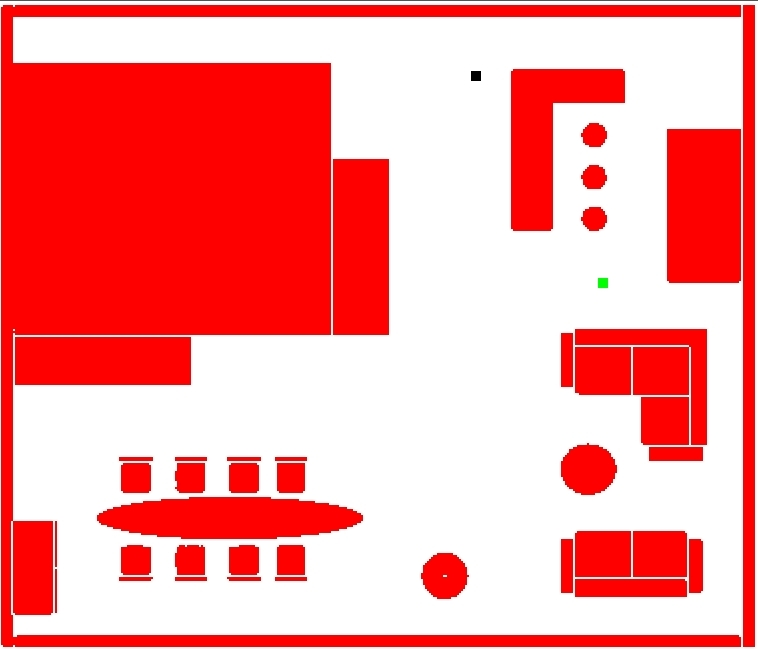
\includegraphics[width=.95\linewidth]{figures/obs_width_2_total_obs_51348.jpg}
		\caption{Obstacle width: 2, number of obstacles: 51348}
		\label{fig:obsmap_sfig2}
	\end{subfigure}%
\end{figure}

\vfill
\begin{figure}[!h]\ContinuedFloat
	\begin{subfigure}[b]{.5\textwidth}
		\centering
		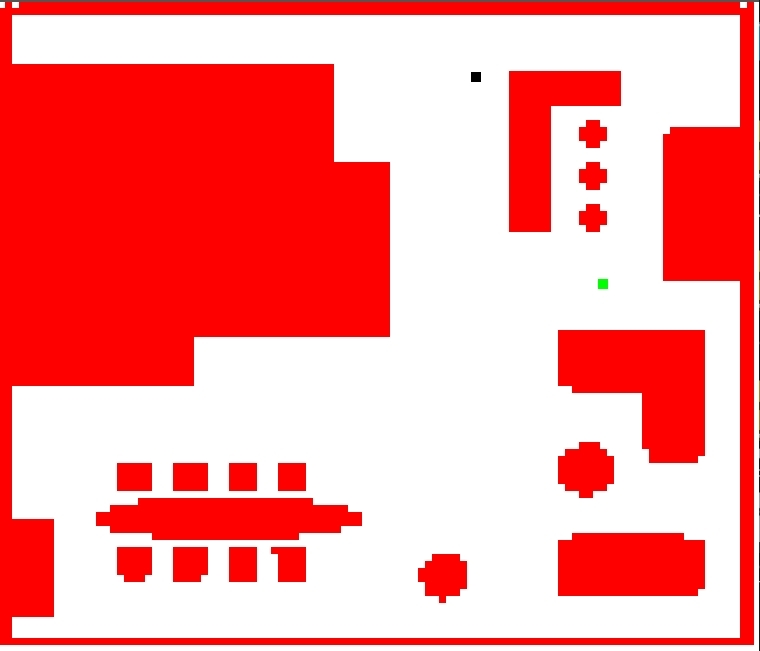
\includegraphics[width=.95\linewidth]{figures/obs_width_7_total_obs_4293.jpg}
		\caption{Obstacle width: 7, number of obstacles: 4293}
		\label{fig:obsmap_sfig3}
	\end{subfigure}
	\begin{subfigure}[b]{.5\textwidth}
		\centering
		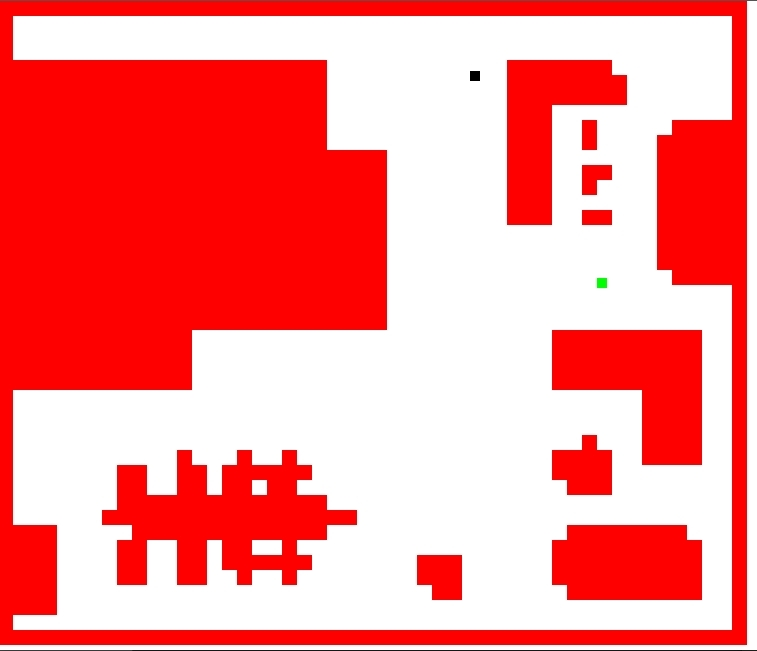
\includegraphics[width=.95\linewidth]{figures/obs_width_15_total_obs_996.jpg}
		\caption{Obstacle width: 15, number of obstacles: 996}
		\label{fig:obsmap_sfig4}
\end{subfigure}
	\caption{Recreation of the given image in the form of an obstacle map in the environment at different resolutions.}
	\label{fig:fig}
\end{figure}


\item \textbf{Annotation file}: It is used to populate the environment with dynamic obstacles. The annotation files contain frame-by-frame details of the position of all the entities of the environment at any given time step. 

\begin{figure}[htbp]

		\centering
		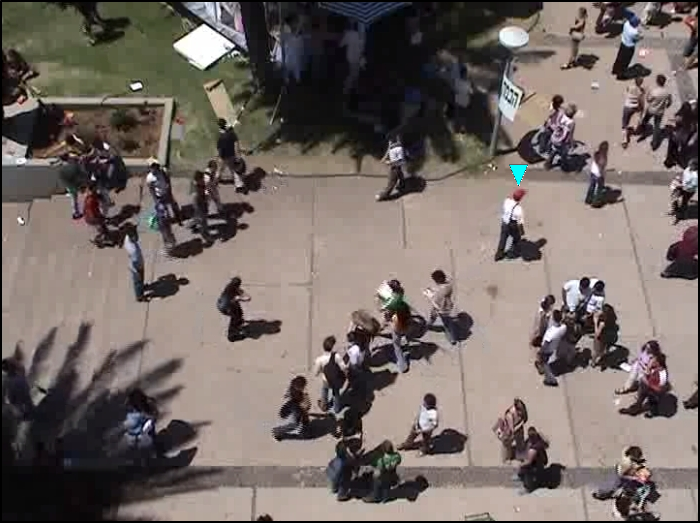
\includegraphics[width=.95\linewidth]{figures/video_frame_students_with_agent_pointer.png}
		\caption{Frame from the original video}
		\label{fig:anno_sfig1}
\end{figure}
\vfill
\begin{figure}[htbp]
		\centering
		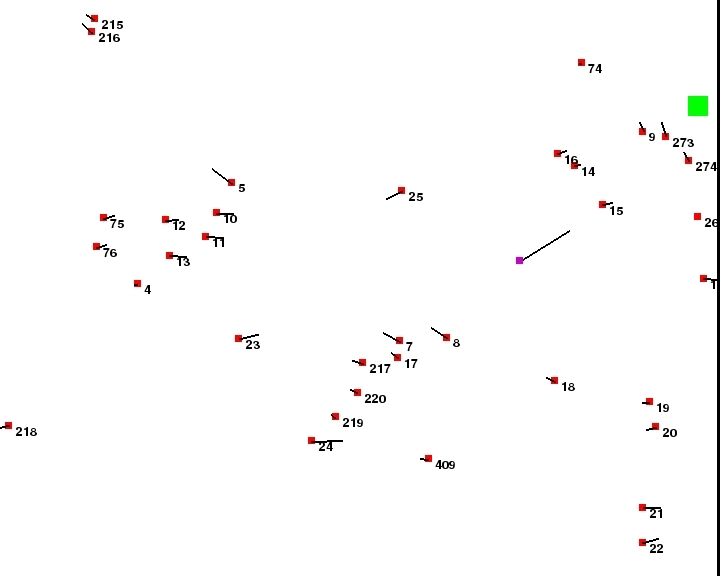
\includegraphics[width=0.9\linewidth]{figures/env_screenshot.jpg}
		\caption{Corresponding frame recreated in the environment using the annotation file.}
		\label{fig:anno_sfig2}

\end{figure}
\end{enumerate}


\subsection{Input spaces and observation (Re-edited entirely)} 
\label{subsec:action-space}
The environment has provisions for both discrete and continuous action space.
\begin{enumerate}
    \item \textbf{Continuous action space}: In this mode, the agent receives two separate inputs controlling its change in speed and orientation. This, along with the current state of the agent is used to compute the position, velocity, and orientation of the agent for the next state as shown in \autoref{eq:next_state_agent} and \autoref{eq:next_state_agent2}.\\
%   \begin{align}
%	\nabla_{orient} & = \texttt{action}_{0}\\
%	\nabla_{speed} & = \texttt{action}_{1}
%	\end{align}
%    where $S_{max}$ is the maximum speed of the agent and $\nabla_{orient}$ and $\nabla_{speed}$ are the change in orientation and speed at a given step respectively.
    
    \item \textbf{Discrete action space}: This mode makes a single choice over a set of predefined actions that control the speed and orientation of the agent. In the current version, the rate of change in speed and orientation is divided into $7$ and $5$ bins respectively thus allowing the agent to take one out of the $35$ predefined actions made from the combination of the two factors. The underlying control is similar to that of the continuous mode.\\
%    \begin{align}
%	    \nabla_{orient} & = \texttt{Arr}_{orient}[\texttt{act}_{t}\%7]\\
%	    \nabla_{speed} & = \texttt{Arr}_{speed}[\texttt{act}_{t}/7]   
%    \end{align}
%    where $\texttt{act}_{t} \in \mathbb{Z} [ 0, 35]$, $\texttt{Arr}_{orient}$ is the orientation array and, $\texttt{Arr}_{speed}$ is the speed array.\\
    The speed and orientation of the agent is updated at every time step using \autoref{eq:next_state_agent}
    \begin{align}
		\label{eq:next_state_agent}
		%\texttt{speed}_{t+1} & =\texttt{min\{} \texttt{max\{(}\texttt{speed}_{t} + \texttt{action}[0]\texttt{), 0\}, } S_{max}\}\\
		v_{t+1} & = \{ {v}_{t} + \delta_{v} :  0 \le v_{t+1} \le S_{max} \}\\
		\label{eq:next_state_agent2}
		%\texttt{orient}_{t+1} & = (\texttt{orient}_{t} + \texttt{action}[1]) \% 360
		o_{t+1} & = \{ {o}_{t} + \delta_{o} :  0^{\circ} \le v_{t+1} \le 360^{\circ}\}
	\end{align}
	where, $v_{i}$ and $o_{i}$ are the speed and orientation of the agent at time step $i$, $\delta_v$ and $\delta_{o}$ are the change in speed and orientation the agent is subjected to at a given time step, and, $S_{max}$ is the maximum permitted speed of the agent. The speed of the agent is measured in pixels per frame.\\ 
	The permitted range of the rate of change in speed and orientation are summarized in \autoref{tab:env_kinematic_ranges}.
\begin{table}[tbhp]
	\begin{center}
		\begin{tabular}{|c|c|c|}
			\hline
			Motion component & Lower bound & Upper bound\\
			\hline
			\hline
			Change in speed per time step & $-0.4$ &  $+0.4$ \\
			Change in orientation per time step & $30^{\circ}$ anti-clockwise & $30^{\circ}$ clockwise\\
			Speed & 0 & 2\\
			Orientation & $0^\circ$ & $360^{\circ}$\\
			\hline
		\end{tabular}
	\end{center}
	\caption{Valid ranges of different motion components of the environment.}
	\label{tab:env_kinematic_ranges}
\end{table}
\end{enumerate}

\subsubsection{The Observation:}
\edited{The observation from the environment returns a tuple of 4 elements: ( $S$, $\rho$, $\mathbf{d}$, $\iota$ ), where
$S$ is the state of environment containing the information relating to the agent, goal, and the obstacles for a given time step,
$\rho$ is the reward obtained at a given time step, $\mathbf{d}$ is a Boolean flag that indicates the completion of the current episode, and $\iota$ contains any extra information the environment might want to convey. }
\subsection{Additional features}
Additionally, the environment comes with a set of options that provide added flexibility and customization while training and evaluating IRL agents.
\subsubsection{Training modes:}
The environment supports 3 types of training modes:. 
\begin{enumerate}
    \item \textbf{Fixed respawn:} The starting and goal position of the agent remains the same throughout the training process.
    \item \textbf{Random respawn:} For every episode, the agent and the goal spawn at random positions on the map. 
    \item \textbf{Replace a pedestrian:} For every episode, the agent assumes the role of a randomly selected pedestrian. Once a pedestrian is selected, the pedestrian is ignored as an obstacle for that episode. The initial position of the agent is set to the coordinated of the pedestrian in its first frame of appearance. Similarly, the goal is set to the coordinates of the pedestrian in the final frame.
    This mode is especially useful for training IRL models because demonstrations from experts for navigation are the optimal demonstrations for a particular configuration of goal and obstacle. Placing the agent in the exact context enables the agent to observe the same state distribution as the expert, which helps to maintain the effectiveness of the expert demonstrations. 
\end{enumerate}
Features available for testing of the environment:
The environment was designed primarily for the development of IRL methods for navigation, and also comes with built-in tools to test IRL methods.
\subsubsection{Deployment of ghost}
IRL agents learn from demonstrations. Creating meaningful metrics to evaluate their performance is elusive, which is why we resort to using IRL in the first place. One simple and effective way of conducting a performance analysis would be to subject the agent to the same conditions as the expert and compare and contrast their behaviors. This is exactly what the environment facilitates. \edited{We define the 'ghost' of a given pedestrian as an entity that traces the exact path, both spatially and temporally, as the pedestrian without interacting or interfering with any other entities of the environment. This greatly benefits in the comparison of the performance of the agent to the expert. }

\subsubsection{User control}
\edited{The environment also has a provision to let an external user control and agent and navigate the crowds. There might be cases where there are not enough expert demonstrations available to perform proper training. In that case, the size of the expert demonstration set can be bolstered by letting humans take control of the agent and generate additional expert demonstrations. }

%The agent can be controlled by a mouse pointer and action is registered only at the time of the click of the left mouse button. Once a click is registered on the map, the direction and magnitude of the vector joining the current position and the location of the click are taken as the desired orientation and speed respectively.  
%The orientation action is then calculated based on the difference between the current orientation of the agent and comparing that with the desired direction. If there is a difference between the two, and a change in the current heading direction of the agent is warranted, then the action to inflict the change is then decided based on the magnitude and sign of the change needed relative to the current heading direction of the agent to minimize the difference.
%The speed action is also calculated in a similar manner, where the magnitude of the difference vector is treated as the desired speed, and based on the current speed of the agent action is taken to minimize the difference.

\subsubsection{Custom scene generation}
The environment has provisions to create custom dynamic scenarios, where the motion of each of the pedestrians can be predefined. This is a very handy tool for creating and testing the agents in situations that are hard to come across or simply unavailable in the available data sets.\\



